\section{W-mass}
\label{sec:w-mass}
With the finished calibration, the mass of the W-boson can now be measured. 
In order to determine the W-mass, we use a data set of actual ATLAS data containing $W \rightarrow e\nu$ events,
as well as several simulated data sets also containing $W \rightarrow e\nu$ events. 
There is also a $Z^0 \rightarrow e^+e^-$ data set to check the validity of the previous calibration. Finally there are data sets for QCD- and non-QCD background events.

\subsection{Electron Calibration Verification}

\begin{figure}[H]
    \centering
    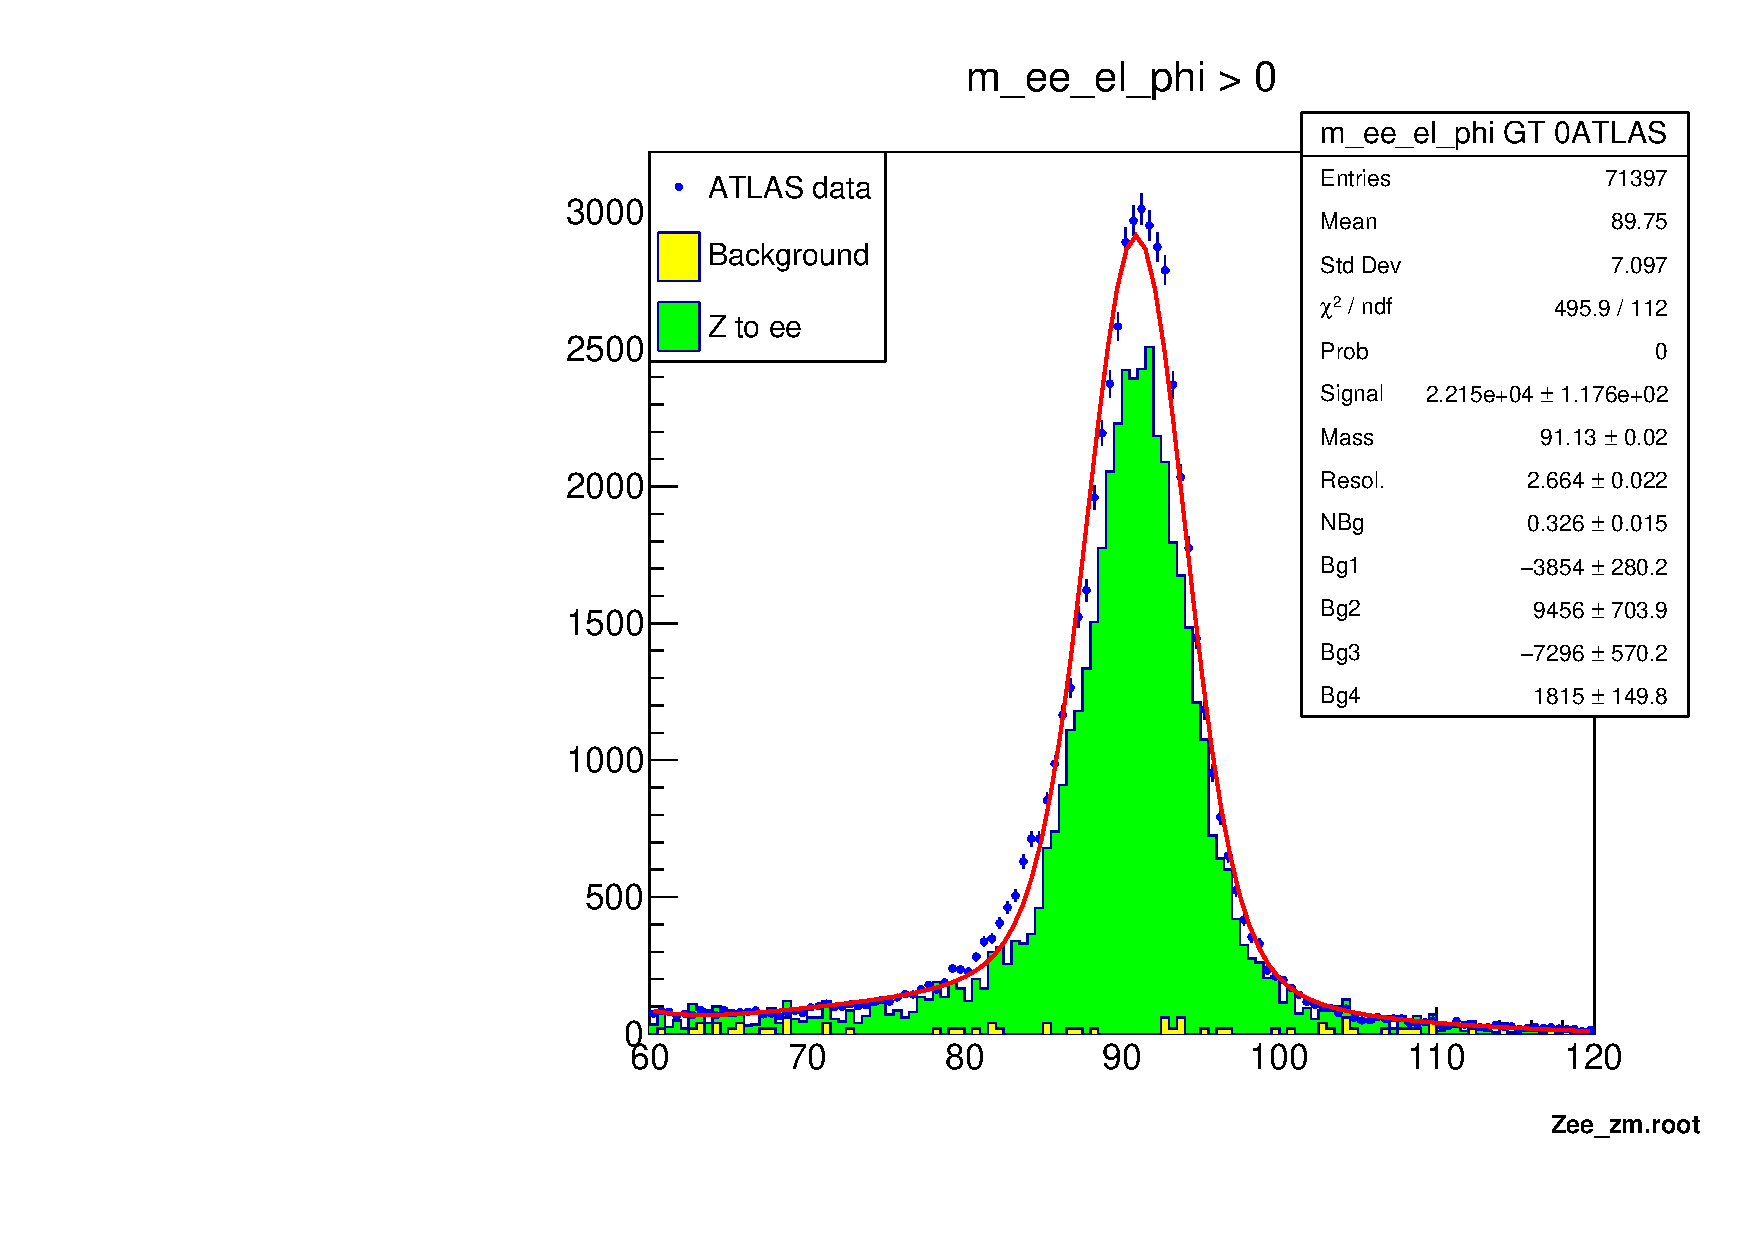
\includegraphics[width=0.7\textwidth]{../W_mass/Z_mass_check_phi_positive.pdf}
    \caption{$Z_mass_check_el_pt-cut.pdf$}
    \label{fig:z-mass_check}
\end{figure}

\begin{table}
    \centering
    \begin{tabular}{ccc}
        \toprule
        \toprule
        cut selection & $M_{Z^0,meas}$ / GeV & $\bigl| \frac{M_{Z^0,meas}- M_{Z^0,lit}}{M_{Z^0,meas}} \bigr|$ \\
        \midrule
        $p_{T,e^{\pm}} > 40$ GeV & $91.71 \pm 0.02$ & \\
        $p_{T,e^{\pm}} < 40$ GeV & $90.5 \pm 0.0$ & \\
        $35 < p_{T,e^{\pm}} < 55$ GeV & $91.43 \pm 0.02$ & \\
        $\eta > 2$ & $89.89 \pm 0.05$ & \\
        $\eta < 0.5$ \& $p_{T,e^{\pm}} > 40$ & $91.69 \pm 0.02$ & \\
        $\eta < 0.5$ \& $p_{T,e^{\pm}} < 40$ & $90.56 \pm 0.03$ & \\
        $\phi < 0$ & $91.14 \pm 0.02$ & \\
        $\phi > 0$ & $91.13 \pm 0.02$ & \\
        \bottomrule
        \bottomrule
    \end{tabular}
    \caption{Measured $Z^0$ mass for different cut selections}
    \label{tab:z-masses}
\end{table}


\subsection{QCD scale factor}

\subsection{Cut selection}

\subsection{Gauge curves}

\subsection{W-mass }